





% \section{Problem Statement}
\section{Background}
\label{sec:methods}

% \subsection{Task and Background} 
\label{sec:task_description}
\label{sec:task}
% We seek to understand how transformers solve the task of 
% \textit{indirect object identification} (IOI), depicted on the left of Figure \ref{fig:directed_graph_figure}. 

In this section, we introduce the IOI task, review the transformer architecture, define circuits more formally, and describe a technique for ``knocking out'' nodes in a model. % knockouts. 

% Arthur comment out old paragraph
% \textbf{Task description.} In indirect object identification (IOI), two names (the indirect object (IO) and the first occurrence of the subject (S1)) are introduced in an initial dependent clause (see Figure \ref{fig:directed_graph_figure}). A main clause then introduces the second occurrence of the subject (S2), who is usually exchanging an item. The task is to complete the main clause, which always ends with the token `to', with the non-repeated name (IO). We create many dataset samples for IOI using 15 templates (see Appendix \ref{app:templates}) with random single-token names, places and items. We use the notation $\pioi$ for the distribution over sentences generated by this procedure.
% end comment out old paragraph

\textbf{Task description. } A sentence containing indirect object identification (IOI) has an initial dependent clause, e.g ``When Mary and John went to the store'', and a main clause, e.g ``John gave a bottle of milk to Mary''. The initial clause introduces the indirect object (IO) ``Mary'' and the subject (S) ``John''. The main clause refers to the subject a second time, and in all our examples of IOI, the subject gives an object to the IO. The IOI task is to predict the final token in the sentence to be the IO. We use ‘S1’ and ‘S2’ to refer to the first and second occurrences of the subject, when we want to specify position. We create dataset samples for IOI using 15 templates (see Appendix \ref{app:templates}) with random single-token names, places and items. We use the notation $\pioi$ for the distribution over sentences generated by this procedure.

% We made a dataset of IOI in several contexts, which consists of sentences like that in Figure \ref{fig:directed_graph_figure}, with the indirect object (\textbf{IO}) token appearing once in the context and the subject (\textbf{S}) token appearing twice (the two occurences are denoted \textbf{S1} and \textbf{S2}). We use 15 sentence `templates' that have slots for the two names, a place that acts as the setting of the sentence, and an item that the two names exchange. We create a large number of dataset examples by randomising the names, places and items. We call this distribution $\bm{\pioi}$.

% OLD PARAGRAPH 
% Indirect object identification (IOI), as depicted on the left of Figure \ref{fig:directed_graph_figure}, requires choosing the correct name as an indirect object in a sentence, i.e. the sentence “When Mary and John went to the store, John gave a drink to” should be completed with the name “Mary”. %Importantly, the IO has to already be a name in the context, and it can’t be the main clause’s subject (S2) because “John gave a drink to John” does not make any sense. 
% In indirect object identification (IOI), as depicted on the left of Figure \ref{fig:directed_graph_figure}, two names are introduced in an adverbial clause (``When John and Mary...'') or a separate sentence (``Then, John and Mary..."), one of which is also the subject of the main clause. The task is then to complete the sentence with the non-repeated name. We created a dataset of examples by constructing 15 sentence templates and inserting random single-token names, places and objects (see Appendix \ref{app:dataset} for details). We refer to the resulting task distribution as $\pioi$.
% END COMMENT OUT OLD PARAGRAPH

To quantify GPT-2 small's performance on the IOI task, we use two different metrics: logit difference and IO probability. \emph{Logit difference} measures the difference in logit value between the two names, where a positive score means the correct name (IO) has higher probability. \emph{IO probability} measures the absolute probability of the IO token under the model's predictions. Both metrics are averaged over $\pioi$. Over 100,000 dataset examples, GPT-2 small has mean logit difference of 3.56 (IO predicted over S 99.3\% of the time), and mean IO probability of 49\%. %assigns more probability to IO than S, giving 49\% probability to IO and an average logit difference of 3.55. %final output probability distribution, indicating the degree to which the IOI computation dominates other mechanisms  that push for different tokens (i.e. pronouns or articles). 
% GPT-2 small has 49\% IO probability metric and also on over 100,000 dataset examples, it assigns higher logits to IO than S.

% \begin{figure}[H]
% \begin{comment}
% \begin{myequation}
% \text{When }\underset{\textcolor{blue}{\text{IO}}}{\text{Mary}}\text{ and }\underset{\textcolor{red}{\text{S}}}{\text{John}}\underset{\textcolor{black}{\text{S + 1}}}{\text{ went}}\text{ to the }\underset{\text{PLACE}}{\text{store, }} \underset{\textcolor{red}{\text{S2}}}{\text{John}}\text{ gave a }\underset{\text{OBJECT}}{\text{drink} }\underset{\textcolor{black}{\text{END}}}{\text{to}}\underset{\textcolor{blue}{\text{(IO)}}}{\text{Mary}}
% \end{myequation}
% \end{comment}
% 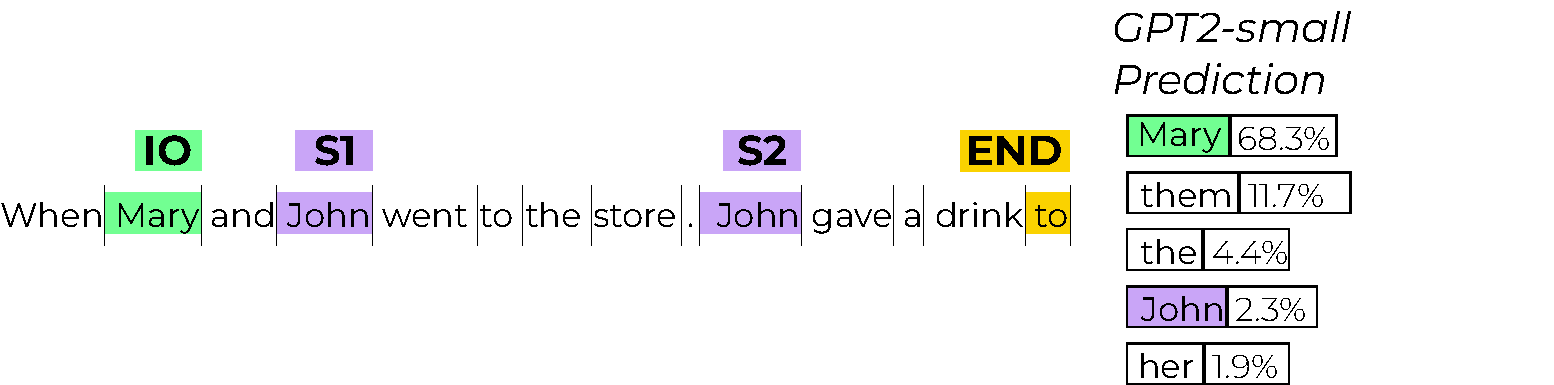
\includegraphics[width=\textwidth]{figs/ioi_task_fig.pdf}
% \caption{An example sentence in our Indirect Object Identification (IOI) task dataset and GPT-2 small top 5 next token prediction. Each template has randomized \textcolor{io_color}{IO}, \textcolor{s_color}{S}, place and object tokens ('store' and 'drink' in the example). Our synthetic dataset consists of sentences with the order \textcolor{io_color}{IO} \textcolor{s_color}{S} \textcolor{s_color}{S} \textcolor{io_color}{IO} and \textcolor{s_color}{S} \textcolor{io_color}{IO} \textcolor{s_color}{S} \textcolor{io_color}{IO} which spans all possible orderings of the two names.
% \label{fig:IOandSandsentence}
% \end{figure}


\textbf{Transformer architecture.} 
GPT-2 small is a decoder-only transformer with 12 layers and 12 attention heads per attention layer. In this work, we mostly focus on understanding the behavior of attention heads, which we describe below using notation similar to \citet{elhage2021mathematical}. We leave a full description of the model to Appendix \ref{app:notation}. 
% In a transformer, input embeddings are modified by attention heads and MLP layers through residual connections. These intermediate activations are known as the \textit{residual stream}, which is projected to the vocabulary  at the end of the forward pass.

The input $x_0$ to the transformer is a sum of position and token embeddings and lies in $\mathbb{R}^{N \times d}$, where $N$ is the number of tokens in the input and $d$ is the model dimension. This input embedding is the initial value of the \textit{residual stream}, which all attention layers and MLPs read from and write to. Attention layer $i$ of the network takes as input $x_{i} \in \mathbb{R}^{N \times d}$, the value of the residual stream at layer $i$. The attention layer output can be decomposed into the sum of {attention heads} $h_{i, j}$. If the output of the attention layer is $y_i = \sum_j h_{i, j}(x_i)$, then the residual stream is updated to $ x_i + y_i$.

Focusing on individual heads, each head $h_{i,j}$ is parametrized by four matrices $W_Q^{i,j}$, $W_K^{i,j}$, $W_O^{i,j} \in \mathbb{R}^{d \times \frac{d}{H}}$ and $W_V^{i,j} \in \mathbb{R}^{\frac{d}{H} \times d}$. 
We rewrite these parameters as low-rank matrices in $\mathbb{R}^{d \times d}$: $W_{OV}^{i,j} = W_O^{i,j} W_V^{i,j}$ and $W_{QK}^{i,j} = W_Q^{i,j} (W_K^{i,j})^T$. The QK matrix is used to compute the attention pattern $A_{i, j} \in \mathbb{R}^{N\times N}$ of head $(i, j)$, while the OV matrix determines what is written into the residual stream. At the end of the forward pass, a layer norm is applied before the unembed matrix $W_U$ projects the residual stream into logits.

% \footnote{This follows \citep{elhage2021mathematical} in that it does not concatenate the attention head outputs and then multiply by the $W_O$ matrix, as this concatenation step can be avoided. This is not a computationally efficient formulation but makes for easier interpretation of the operations.}
%\footnote{Note this explanation in following (\cite{elhage2021mathematical}) does not concatenate the attention head outputs then multiply by the $W_O$ matrix, as this concatenation step can be avoided. This is not a computationally efficient formulation, it was proposed to help the interpretation of the operations.}: 
% if $y_i = \sum_j h_j(x_i)$, then the residual stream is set to $x_i + y_i$ after being fed through the attention module. Finally, the unembed matrix $W_U$ projects the residual stream into logits (after a final layer norm).

% $Attn(X) = X + \sum_{i=1}^{H} h_i(X)$

% Each \textbf{MLP layer} $m$ takes input $x \in \mathbb{R}^{N \times d}$ from the residual stream, and after being passed through a single hidden layer, writes back into the residual stream, so $x + m(x)$ is the new state of the residual stream after a MLP module. 

% \subsection{Explanation Criteria}
\subsection{Circuits and Knockouts}
\label{sec:circuits}
\label{sec:knockouts}

In mechanistic interpretability, we want to understand the correspondence between the components of a model and human-understandable concepts. A useful abstraction for this goal is \emph{circuits}. If we think of a model as a computational graph $M$ where nodes are terms in its forward pass (neurons, attention heads, embeddings, etc.) and edges are the interactions between those terms (residual connections, attention, projections, etc.), a circuit $C$ is a subgraph of $M$ responsible for some behavior (such as completing the IOI task). % A model behavior is a coherent pattern between inputs and outputs (i.e. closing open parentheses with closed parentheses). 
This definition of a circuit is more coarse-grained than the one presented in \citet{olah2020zoom}, where nodes are {features} (meaningful directions in the latent space of a model) instead of model components. 

% Flow
% - motivate mechanistic interpretability again
% - define what a behavior and task is (a pattern between input-output mappings)
% - define what a circuit is and why it's good
% - explain that we map a behavior to a circuit via knockouts and a metric for the behavior
% - don't mention MLP stuff rn
% Inspired by previous work \cite{olah2020zoom}, we define a \textbf{circuit} $C$ as subgraph of the model's entire  computational graph $M$ which implements a behavior. Behavior of a computational subgraph $C$ is defined by \emph{knocking out} all nodes in $M \backslash C$ (see Section \ref{sec:knockouts}). Our circuit is a sparse subset of attention heads at positions in the sentence, while the MLP layers are always fully functional.  However, we empirically find that all layer norms and MLPs except for the first MLP are not important: knocking them out causes little change to the logit difference (Appendix \ref{app:mlp}). 

% OLD VERSION OF THIS PARAGRAPH
% More formally, let $M$ be the set of all nodes in a model (i.e. all attention heads and MLP layers in a transformer). We represent a circuit as a subset $C \subseteq M$. The behavior of a circuit $C$ is obtained by \emph{knocking out} all nodes in $M \backslash C$. We describe the knockout process in detail in Section \ref{sec:knockouts}; for now think of it as removing nodes and running a forward pass on the remaining nodes.
% END OLD VERSION

% To formalise this, let our model $M$ be a computational graph, where nodes are components of the model (neurons, attention heads, etc.) and edges the dependencies defined by the model architecture. We define a circuit as an induced subgraph of $M$. This definition is slightly different from \cite{olah2020zoom}'s definition of circuits, where nodes are \textit{features}, meaningful directions in the latent space of a model, and edges are defined by the model's weights. This is because we want $C$ to describe the end-to-end behavior of a language model, rather than completely explain the early layers of a vision model. Behavior of a computational subgraph $C$ is defined by \emph{knocking out} all nodes in $M \backslash C$. %We describe the knockout process in detail in Section \ref{sec:knockouts}; for now think of it as removing nodes and running a forward pass on the remaining nodes.

% MOVING CRITERIA TO A DIFFERENT PLACE START
% Before moving forward, we define criteria for what constitutes a ``good'' explanation. Intuitively, a good circuit should not just achieve high accuracy on the IOI task, it should also do so in the same way that GPT-2 itself does. We define three criteria below--faithfulness, completeness, and minimality--that help ensure this. In addition, the circuit should be \emph{legible}--we should understand what each component does.


% \textbf{Explanation Criteria.} 
% Let $F$ be a metric that measures performance on a task: in our case, $F$ is the logit difference.

% Our first criterion,  \textbf{faithfulness}, requires that $C$ achieve similar performance under the metric as the entire model $M$:
% , i.e. we want the absolute difference $|F(C) - F(M)|$, called the \emph{faithfulness score}, to be low.
% \begin{definition}
% \label{def:faithfulness}
% A circuit $C$ is $\varepsilon$-faithful if 
%\begin{equation}
%   \text{ \textbf{Faithfulness}: } 
% $|F(C) - F(M)| \leq \varepsilon$. 
%\label{eqn:faithfulness}
%\end{equation}
% \end{definition}
%that the model has low \textit{faithfulness score} $|F(C) - F(M)|$.

% However, a faithful circuit may be inadequate as an explanation for model behaviour. For instance, if the model uses two similar, serial circuits $C_1$ and $C_2$ in parallel before applying an OR operation to their results, identifying only one of them is enough to achieve faithfulness. But in this case, we would like to identify both circuits present in $M$.

% To resolve the issue that $C$ may compute an algorithm in $M$ using a different set of nodes to $M$, we need introduce a new criterion. Knocking out the same set of nodes $K$ from $C$ and $M$ should lead to the same effect on model performance, measured by $F$.

% We formalized this intuition by introducing the \textbf{completeness} criterion:

% NEW COMPLETENESS
% \begin{definition}
% A circuit $C$ is $\varepsilon$-complete if\footnote{$K$'s are uniformly sampled from all subsets of $C$} $\mathbb{E}_{K \subseteq C} [ |F(C \setminus K) - F(M \setminus K)| ] \leq \varepsilon$.
% \label{eqn:completeness}
% \end{definition}
% END NEW COMPLETENESS

% OLD COMPLETENESS SECTION
% \begin{definition}
% A circuit $C$ is $\varepsilon$-complete if $\forall K \subseteq C, |F(C \setminus K) - F(M \setminus K)| \leq \varepsilon$. 
% \label{eqn:completeness}
% \end{definition}
% END OLD COMPLETENESS CRITERION

% In the previous example, if $C = C_1$ and $K=C_1$, $C \setminus K$ will be the empty circuit while $M\setminus K$ will still contain $C_2$. In this case $|F(C \setminus K) - F(M \setminus K)|$ will be large, and thus the partial explanation will not pass the completeness test. We give an example of a faithful but incomplete circuit in Section \ref{sec:validation}, but note that this definition doesn't cover all cases\footnote{If two nodes in $M \setminus K$ perfectly cancel each other, independent from $C$ then the completeness definition could be met without including either of these important nodes in a circuit. We could also check that $\mathrm{F(C)}$ doesn't change after adding nodes: $\forall K \subseteq M, |F(C \cup K) - F(M)| \leq \varepsilon.$ However, in practice such cases of compensation are improbable.} .


% A faithful and complete circuit may contain unnecessary components, and so be overly complex. %For instance, $M$ is a faithful and complete circuit but doesn't give any interpretability insights because it contains nodes irrelevant for the behavior. For a circuit to be a useful explanation, 
% To avoid this, we should check that each of its nodes $v$ is actually necessary. %has a counterfactual impact on $F$. 
% This can be evaluated by showing that $v$ can significantly recover $F$ after knocking out a set of nodes $K$: we justify why this set formalism is required after giving the definition of \textbf{minimality}:
% \begin{definition}
% A circuit $C$ is $A$-minimal if  $\forall v \in C, \exists K \subseteq C, |F( (C \setminus K) \cup \{v\}) - F( (C\setminus K))| \geq A$.
% \label{eqn:minimality}
% \end{definition}
% This formulation importantly captures the case of redundant computation introduced earlier. To show that the circuit $C = C_1 \cup C_2$ is minimal, we first show that for $v_1 \in C_1 \setminus C_2$ and $K = (C_2 \setminus C_1) \cup v_1$, $|F((C \setminus K) \cup v_1 ) - F( (C\setminus K))| = |F(C \setminus C_2) - F( C\setminus (C_2 \cup v_1))|$ is large, since $C_1$ is a serial circuit, removing $v_1 \cup C_2$ will destroy the behavior. We then proceed symmetrically for $v_2 \in C_2$.

%However, a complete circuit may still not be `correct' as an explanation, and we would want to make it as small as possible while still being complete. \todo{can extend this?}
% \begin{comment}
% \begin{itemize}
% \item \textbf{Minimality}: a circuit is minimal if 
 
% \begin{equation}
%     \forall v \in C, \exists K \subseteq C, |F( (C \setminus K) \cup \{v\}) - F( (C\setminus K))| \geq A.
% \label{eqn:minimality}
% \end{equation}
% \end{itemize}
% \end{comment}

% \begin{definition}
% We call the quantity $|F(C) - F(M)|$ the \textit{faithfulness score}, $|F(C \setminus K) - F(M \setminus K)|$ the \texti{completeness score} and $|F( (C \setminus K) \cup \{v\}) - F( (C\setminus K))|$ the minimality score.
% \end{definition}

% Finally, we also wish to understand the actual operations performed by the nodes. We therefore add a qualitative criterion of \textbf{legibility}: every component of $C$ cleanly corresponds to a component of a human-understandable causal model. To check legibility, we provide an explanation of the human-understandable algorithm that $C$ implements and verify this with causal interventions (Section \ref{sec:legibility}). 
% WE'VE MOVED ALL OF CRITERIA

%\subsection{Knockouts}
%\label{sec:knockouts}
% \label{sec:patching}

Just as the entire model $M$ defines a function $M(x)$ from inputs to logits, we also associate each circuit $C$ with a function $C(x)$ via \emph{knockouts}. A {knockout} removes a set of nodes $K$ in a computational graph $M$ with the goal of ``turning off'' nodes in $K$ but capturing all other computations in $M$. Thus, $C(x)$ is defined by knocking out all nodes in $M \backslash C$ and taking the resulting logit outputs in the modified computational graph.
%Suppose $X \sim \pioi$. We define $M(X)$ as the output logits of the network on input $X$. 
%The goal of this section is to define a function $C(x)$ from inputs to logits, for any circuit $C \subseteq M$. We do so by \emph{knocking out} all nodes in $M \backslash C$. 

% A first naïve knockout approach consists of simply deleting each node in $K$ from $M$, which is the same as \textit{zero-ablations} \citep{LeCunAblation} in transformers. This na\"ive approach has an important limitation: 0 is an arbitrary value, and subsequent nodes might rely on the average activation value as an implicit bias term. We find zero-ablations to lead to noisy results in practice.
A first naïve knockout approach consists of simply deleting each node in $K$ from $M$. %Since the residual stream in a transformer is a continual path from input to output (see Section \ref{sec:task_description}), and for us $K$ is always a set of MLPs and attention heads at various sequence positions, this leaves a computational graph so that $M \setminus K$ is well-defined. 
The net effect of this removal is to \textit{zero ablate} $K$, meaning that we set its output to 0. This naïve approach has an important limitation: 0 is an arbitrary value, and subsequent nodes might rely on the average activation value as an implicit bias term. Perhaps because of this, we find zero ablation to lead to noisy results in practice. %Indeed, 0 is an arbitrary value that can be far from the baseline activation of a node $v$ in $K$. The computation of latter nodes from $M\setminus K$ can be highly perturbed because they rely on $v$ being in some ``normal" range. 

To address this, we instead knockout nodes through \textit{mean ablation}: replacing them with their average activation value across some reference distribution, similar to the bias correction method used in \citet{meca_interp_grokking}.  Mean-ablations remove the information that \textit{varies} in the reference distribution (e.g.~the value of the name outputted by a head) but will preserve \textit{constant} information (e.g.~the fact that a head is outputting a name). %Through mean-ablations, we are interested in finding the components that move information about names, which is the core of the IOI task and also varies with the distribution.
%limit the destructive effect of off-distribution activations, we use \textit{knockout} to refer to computing the average activation vector for elements of $K$ across a dataset and then replacing the activations of each element of $K$ with their average vector on the knockout dataset. 

%In this work, all knockouts are performed in a modified distribution with three random names we called $\pabc$ (where A, B and C refer to the three distinct names). In $\pabc$, sentences no longer have a single plausible IO, but the grammatical structures from the $\pioi$ templates are preserved.


In this work, all knockouts are performed in a modified $\pioi$ distribution called $\pabc$. It relies on the same generation procedure, but instead of using two names (IO and S) it used three unrelated random names (A, B and C). In $\pabc$, sentences no longer have a single plausible IO, but the grammatical structures from the $\pioi$ templates are preserved.

We chose this distribution for mean-ablating because using $\pioi$ would not remove enough information helpful for the task. For instance, some information constant in $\pioi$ (e.g. the fact that a name is duplicated) is removed when computing the mean on $\pabc$.

When knocking out a single node, a (head, token position) pair in our circuit, we want to preserve the grammatical information unrelated to IOI contained in its activations. However, the grammatical role (subject, verb, conjunction etc.) of a particular token position varies across templates. To ensure that grammatical information is constant when averaging, we compute the mean of a node across samples of the same template.


%Computing means across the entire distribution instead of templates would average activations from different positions tokens, like names, verbs and conjunctions, mixing information destructively.



% We mean-ablate with respect to this distribution, which we call the `DEF' distribution, to balance the destructiveness of our knockouts. $\pioi$ as a reference distribution would not remove constant information that is helpful for the task, while other distributions would introduce more destructive, off-distribution information.
% In these knockouts, we compute the means for each template across each token position to avoid mixing information of different types of tokens.
% To knockout a single node, a (head, token position) pair in our circuit, we compute the mean of that node across samples of the same template to avoid mixing information.

% if we instead computed means across the entire distribution, computing means across token positions would average activations of different tokens, like names, verbs and conjunctions. 
% like averaging over activations at tokens of both names and verbs. 
% We call this distribution the `DEF' distribution. 
% where A, B and C represent the three distinct names in the sentence. 
% the grammatical function of the words (e.g. the mean activation can contain the fact a token is a name but not the value of any particular name). We call this distribution the `DEF' distribution, where A, B and C represent the three distinct names in the sentence. 

%There are two ways we can remove $K$: we could \textit{zero ablate} $K$ (\cite{ablation_studies}), meaning that we turn its output to 0, or 
%alternatively we could \textit{mean ablate} it. In a mean ablation we compute the average activation vector for elements of $K$ across a dataset of example inputs, then replace the activations with this average vector. 

%perform a forward pass with a large number of dataset examples, sample the activations of $K$, and then perform a second forward pass, setting $K$'s output to the constant mean over these samples.
%Mean ablation usually works better than zero ablation, since a lot of transformer behavior involves copying earlier outputs (\cite{elhage2021mathematical}), and so zero ablating results in exploring off-distribution behavior. 

% A first simple choice is the training distribution. In our case, we compute the activations of network components across many OpenWebText (OWT) (\cite{GPT2}) examples, and then replace some activations in the network with these activations.

% To study more precisely the movement of information in the IOI task, we also used a particular mean ablation that preserves the semantic role of tokens. Contrary to the OWT ablation, the tokens are aligned according to their function in the sentence. For a given module, we compute its mean activation for a given token position and a given template by averging across samples where the IO, S, place and object token of the sentence were randomized (see Section \ref{sec:task}). Because we preserve the template and the token position, the resulting mean still contain the grammatical meaning while removing the exact value of the token. (e.g. the mean activation on the second token can still contain the fact that it's a name while not containing the value of any particular name). This means that performing this type of ablation will not enable us to study the features that are constant in the distribution, such as why some heads pay attention to names.

% We briefly cover the extensions of the results when knockouts are performed with respect to the OpenWebText (OWT) distribution in Appendix \ref{app:owt_knockouts}.


% OLD INTERP TECHNIQUES:
% To study this additional mechanism, we also chose a third baseline distribution that do not have a single plausible IO by replacing the S2 token (i.e `Mary and Kohn went to the store and Chris gave a drink to'), while keeping in-template averages. This way, we can isolate the modules that activate specifically in the case of a single IO, while preserving the grammatical information unrelated to IOI. We called this technique DEF-ablation. 

% As introduced in the previous section, we are interested in isolating the effect of a subcircuit $C \subseteq M$. This experiment, called \emph{circuit extraction}, consists in DEF-ablating every node from $M \setminus C$.

%Within each template sentence for IOI (see Section \ref{sec:task}), we compute the average activations in a particular position over some dataset. Ablation is then the insertion of the average of the activations for a given template and sequence position pair, for some of the components of the model. 

% \begin{figure*}
%     \centering
%     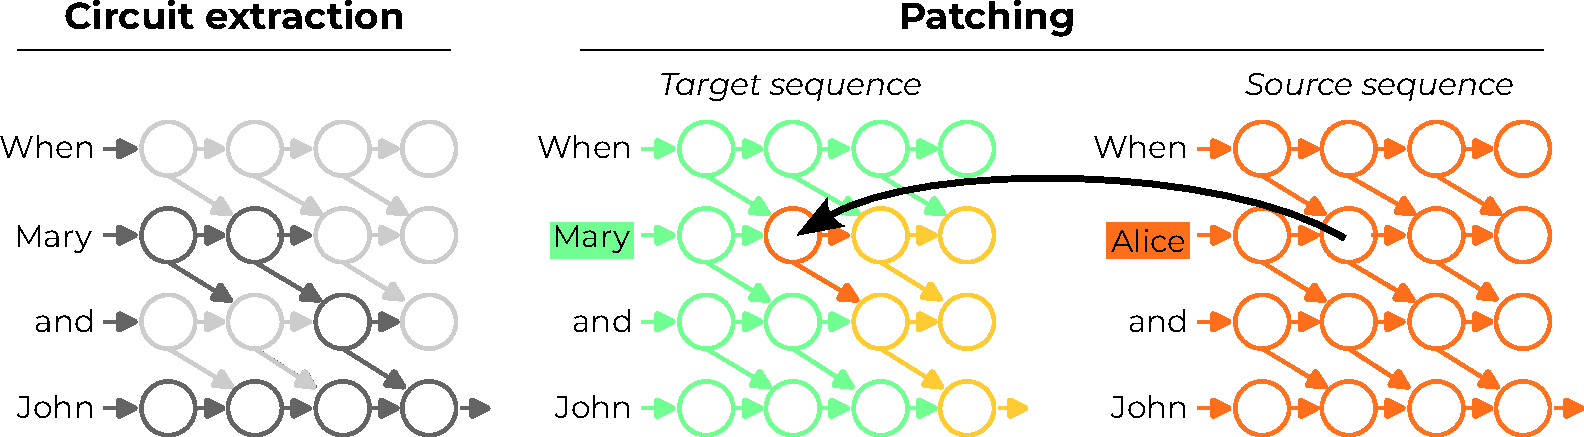
\includegraphics[width=0.8\textwidth]{figs/patching_and_circuit_extraction.pdf}
%     \caption{Illustration of our experimental intervention on activation. \textbf{Left}: circuit extraction \todo{should the circuit should be in green...?}, we knockout every node that is not part of the investigated circuit. \textbf{Right}: patching experiment, we copy the activation from a module on the source sequence to the network processing the target sequence.}
% \label{fig:owt_patch_circuit_discov}
% \end{figure*}

% %The dataset choice is important here, and its choice depends on the effect we want to study. For the most general ablation, we can ablate over the Open Web Text distribution (\cite{GPT2}) that GPT-2 was trained on. However, the generality of this ablation does not always allow for us to isolate behaviours specific to the IOI distribution. We can alternatively ablate over the IOI distribution, where we average activations over the outputs on sentence from (\ref{fig:IOandS}). In this case we are investigating in which way the model is taking advantage of having a non-constant computation at this node compared to having its mean.  

% %We experimentally found advantages and disadvantages with this approach. On one hand, we became able to progress far faster on the discovery side of things, and were able to ignore large parts of the network.
% However, we also found that certain circuit behaviours (e.g the `signal' from section (\ref{sec:overview})) that were constant across the IOI distribution, though not constant in OWT more generally led to `mean ablations' that were not truly ablations in the `removal' sense. To get around this issue, we also fed a number of dataset examples where the S2 token was replaced by a name that was distinct from the IO and S tokens (e.g `Mary and Kohn went to the store and Chris gave a drink to') in order to perform ablations that kept the necessary context of the template for ablations that allowed us to isolate the circuit, while not in fact being examples of indirect object identification. We call this dataset the `DEF' dataset.

% For our purposes, $K$ is always the union of several pairs $(f, \text{IND})$, where $f$ is an attention head or MLP within the network, and $\text{IND}$ refers to an index in the input sentences. This may be either the literal index, position $ \text{IND} \in \{ 0, 1, ... \} $ or alternatively the semantic index $ \text{IND} \in \{ \text{IO}, \text{S}, \text{S1+1}, \text{S2}, \text{END} \} $, or the complements of indices (for example, if $h$ is an attention head, and $K = \{\left(h, \text{IO}^C\right)\}$, then $M \setminus K$ refers to the model with the output of $h$ ablated at all sequence positions except $\text{IO}$). In general, the `dataset' used for mean ablation is template-specific: the average activations used for the sentences of the form `When \IO and \S went to the [PLACE], \STwo gave a [OBJECT] to' is taken over only other sentences of this form (possibly with \IO and \S swapped around), and we do the same for all the other templates. \ac{this section is super long, maybe move to appendix or cut some?} \todo{also explain circuit extration here}

% \krw{here's where i think the section where we explain circuits and mechanistic interp and all that stuff should go, something like:} \ac{That sounds reasonable, if we want this we could just move the intro paragraph 2 here?}
% In mechanistic interpretability, we want to find circuits. circuits are X. we find circuits using a bunch of techniques which we describe, one of which is new. then we motivate each technique by how they help us understand information flow
% The set of techniques we used for finding or validating the circuit including projection, activation patching, ablations and attention pattern analysis. 

%Following the \textit{logit lens} technique (\cite{LogitLens}), we project hidden states along certain directions to identify which nodes in the model are producing outputs that contain information of interest. The logit stream is directly read from and written to by all attention heads and MLPs in the network, so it's natural to study this object to understand network behavior.

% \subsubsection{Activation Patching}
% \label{sec:patching}
% In patching, we compute a forward pass of the network on a \texit{source} distribution, saving all activations computed. We then perform a forward pass on the \textit{target} distribution, replacing some activations with the activations from the source distribution. Activation patching can be viewed as an ablation where the dataset used to sample the activations from is different from the dataset we run the model on, and such a dataset may differ for each of the inputs in the batch of the source distribution. In practice, we use patching as a technique for causal interventions on models to verify or contradict hypotheses. 
%, unlike the attribution and removal use cases of ablation, and so the two serve different purposes.

% an ablation that only ablates directions that are specific to the target distribution. 

% \subsubsection{Attention Pattern Analysis}
% We look at the attention patterns to understand which token positions a given attention head is reading from. Though attention has been shown to be misleading from an interpretability perspective (\cite{attention_not_explanation}) in practice, we find that they are useful for forming hypotheses for the function of circuit components that can later be validated.


% Dataset generation from templates


% OLD EXPLANATION CRITERIA
%To isolate a circuit $C$ from $M$ that computes the behavior, we need metrics that quantify the behavior (logit difference and IO probability in this case) and a method that allows us to evaluate these metrics on a given subgraph $C$. Crucially, this method must enable us to remove the irrelevant nodes $M \setminus C$ without completely destroying model internals. To this end we \textit{knockout} all nodes in $M \setminus C$ (see Section \ref{sec:knockouts}), essentially `extracting' the circuit from the model. Fix some metric $f(x, C(x))$ (e.g.~the logit difference on input $x$), and let $F(C) \eqdef \mathbb{E}_{x \sim \pioi}[f(x, C(x))]$.
%Formally, we quantify behavior as a metric $F: \mathcal{C} \to \mathbb{R}$, where $F(M)$ quantifies the model's normal behavior and $F(C)$ quantifies the circuit's behavior (where knockout is implicitly used to remove the nodes in $M \setminus C$). 
%
% To isolate a circuit $C$ from $M$ that computes the behavior, we need metrics that quantify the behavior (logit difference and IO probability in this case) and a method that allows us to evaluate these metrics on a given subgraph $C$. Crucially, this method must enable us to remove the irrelevant nodes $M \setminus C$ without completely destroying model internals. To this end, we devise \textit{circuit extraction}, a method that knocks out the nodes in $M \setminus C$ and is described in Section \ref{sec:knockouts}). Formally, we quantify behavior as a metric $F: \mathcal{C} \to \mathbb{R}$, where $F(M)$ quantifies the model's normal behavior and $F(C)$ quantifies the circuit's behavior (where circuit extraction is implicitly used to knockout $M \setminus C$). 
%
% In our case, we use logit difference and IO probability. These metrics can be seen as a function $F: \mathcal{C} \longrightarrow \mathbb{R}$ that assigns %
%
% These metrics can be seen as a f\emph{metric} $F: \mathcal{C}_M \longrightarrow \mathbb{R}$ from $\mathcal{C}_M$ denoting the set of circuits in $M$ to $\mathbb{R}$.
%
%
%Let $\mathcal{C}_M$ denote the set of circuits in $M$. Suppose some behavior of the model, such as its ability to predict IO rather than S as the correct token, is reflected in a \textit{metric} . In our work we use the \textit{logit difference}, the average difference between the logits on the IO token and the logits on the S token, as it is large both when the model places a high probability on IO being the correct token, and when it ranks IO as more likely than S.
%
% Given this proxy to describe the behavior, the task of circuit identification can be seen as finding $C$ explaining the best $F(M)$. To concretize this intuition, we would like to evaluate how much $C$ contribute to $F(M)$ by removing every node from $M \setminus C$ in the computation of $F$. The naïve approach of simply removing those nodes is bound to fail, as transformer modules depends on the average values of previous nodes. We discuss how we implemented \emph{circuit extraction} by ablating the node from $M \setminus C$ in more details in \ref{sec:knockout}. This technique enables us to compute $F(C)$ for every $C \subseteq M$.
%
%\av{TODO: talk about ablation and $F(C)$}
%

%must include these additional heads by making sure that the circuit is \textbf{complete}, which we can formalise as $\forall K \subseteq C, |F(C \setminus K) - F(M \setminus K)| \leq \varepsilon$. 

%Here, if $C$ is the circuit that consists only of the heads that increase logit difference in the full model, and we choose $K=C$, then $F(C \setminus K)$ will be close to 0, though $F(M \setminus K)$ will not due to these `backup name movers'. \ac{this final sentence could be cut / be made less detailed but I gave the full picture}

% rip the toy example
% As a toy example, suppose a computer program sets variables $a=1$, $b=0$, $c=0$ and $d=0$ and then outputs the product $a \times b \times c$, and $F$ maps subsets of $M = \{ a, b, c, d\}$ to their product \ac{mention that $F(\emptyset) = 0$ is required for this to check out?}. One could argue i) that the output behavior is explained by $a \times b$ entirely, as this product is 0 as well as the true neural net computation. Alternatively, one could also argue ii) that the network output is explained by $a \times b\times c \times d$ entirely, as this product is also 0. These explanations meet the `faithful' standard for $\varepsilon = 0$, but don't actually explain network behavior. Hence if $\varepsilon, A \in \mathbb{R}$, we consider $C$ to be a $(\varepsilon, A)$-successful explanation if it meets the two further criteria:
% Explanation i) of the multiplication behavior is not complete as here $C = \{ a, b \}$, so letting $K = \{ b,c \}$ leaves $F ( C \setminus K) = 1$, but $F(M \setminus K) = 0$.
% Explanation ii) of the multiplication behavior is not minimal because here $C = \{ a, b, c, d \}$, and $v = d$ does not change the circuit output. 

% \begin{figure*}
% \begin{center}
% 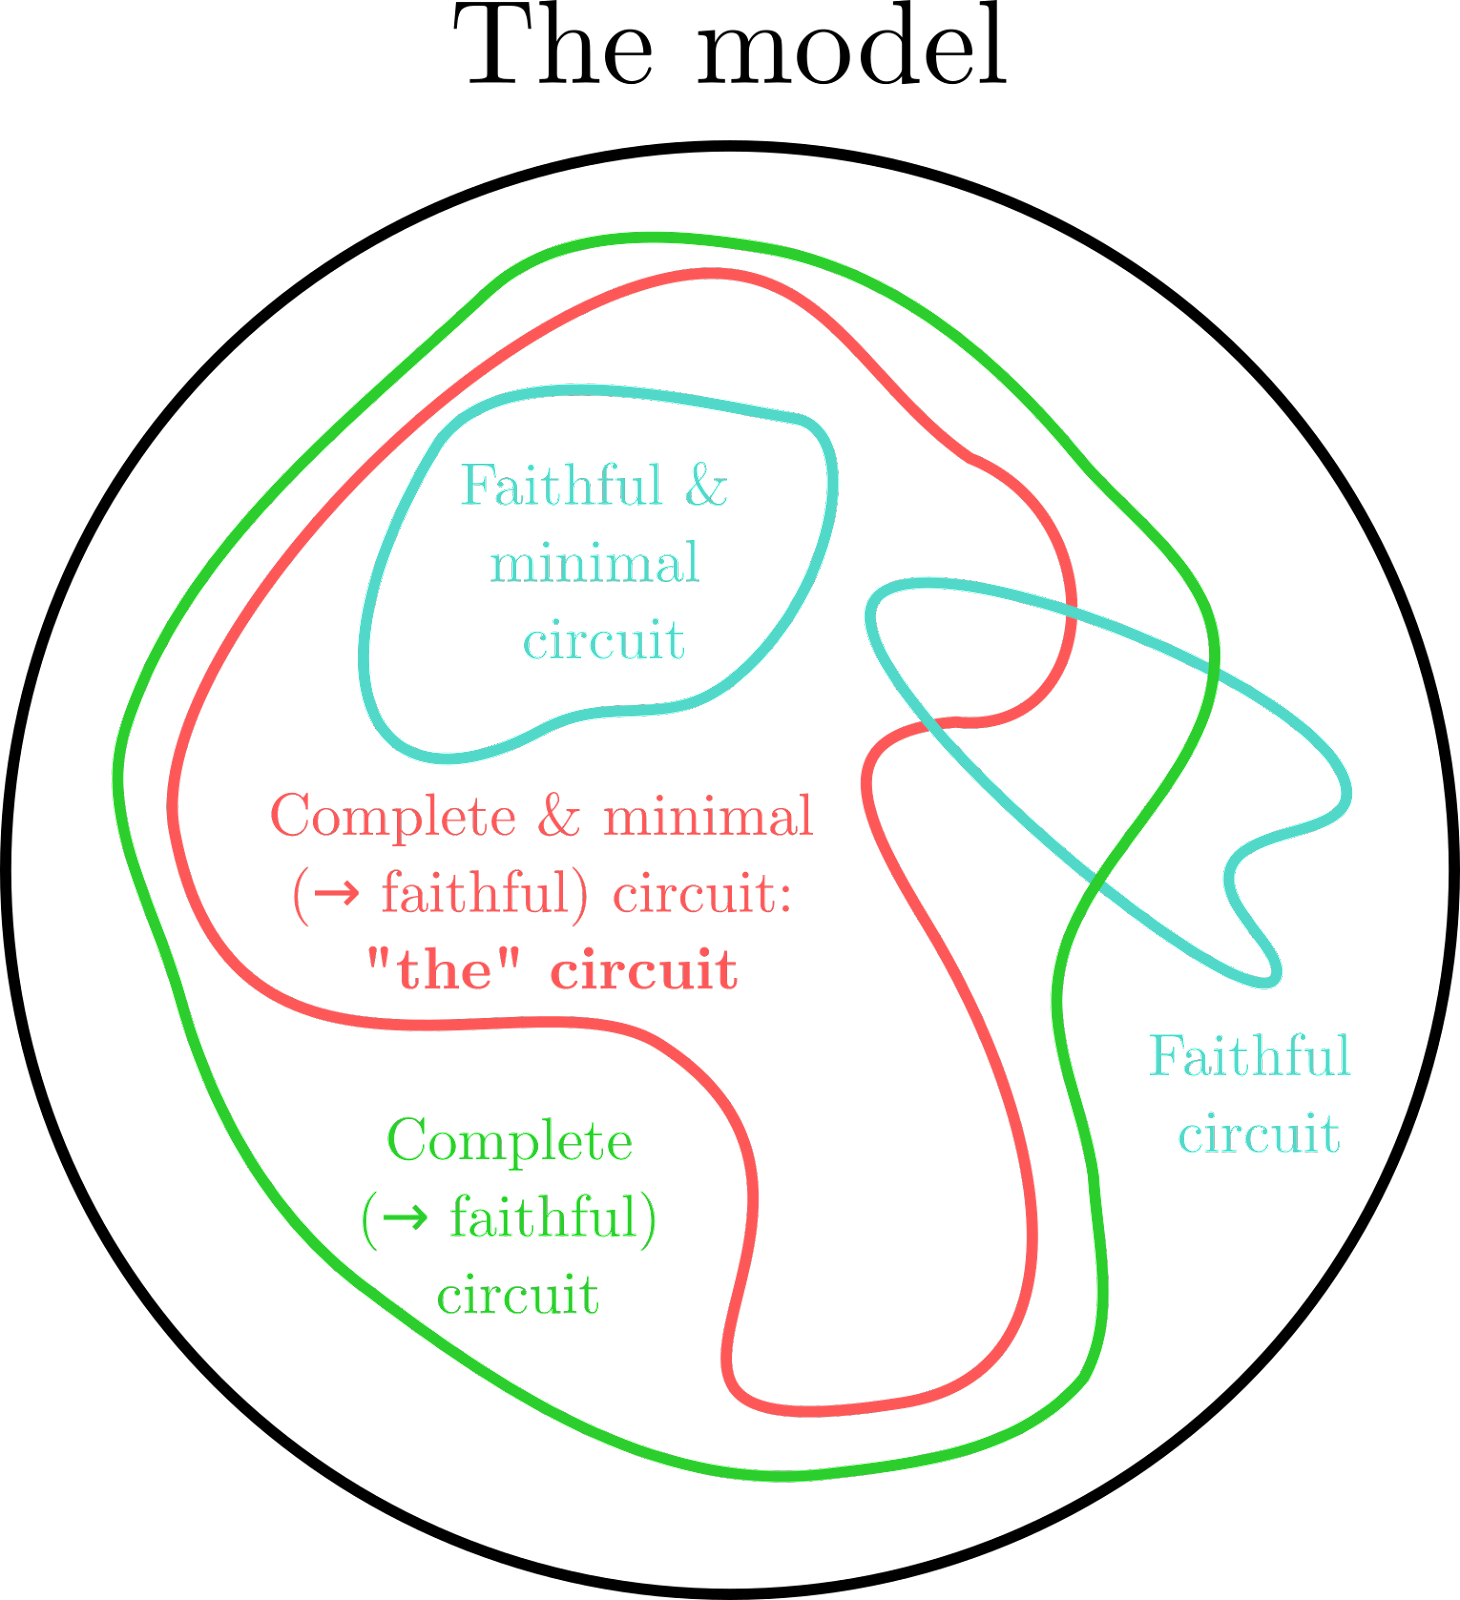
\includegraphics[width=0.4\textwidth]{figs/circuit_decomposition.png}
% \end{center}
% \caption{Illustration of possible circuits that could be found as subsets of the model's nodes.}
% \end{figure*}

% This criterion can be thought as ensuring a level of knowledge similar to what is attained by biology: our understanding is build by thoroughly investigate each parts of $C$ and their interaction through a succession of observation and causal interventions as described in Section \ref{sec:legibility}. However, given the difficulty of encompassing these multifaceted phenomena within a single global quantified criterion, this definition is left defined in these qualitative terms. 


%Finally, it's also important for our circuit to be \textbf{legible}: for its components to cleanly correspond to a human-understandable causal model. This definition is left defined in these qualitative terms, and we explain our understanding in Section \ref{sec:legibility}. 

% We defined this framework to be reasonably rigorous while enabling an empirical evaluation of the proposed criteria. We chose to work with nodes instead of links to limit the combinatorial explosion of elements to investigate while ensuring a reasonable level of understanding. Moreover, the metric $F$ is used as a proxy for the behavior. In general, the task to understand contains different aspect that cannot be summarized in a single function. 
% To validate our work, we choose several different $F$ and verify the criteria for each of them.



% OLD CIRCUIT INTERPRETATION INTRO
% \paragraph{The circuit interpretation:}
%The information flow in transformers can be interpreted as head communicating through the residual stream by writing or reading in subspaces. For instance, the matrix of a head $i$ can use the information written by the earlier head $j$ to change the token $W_{OV}$

% investigating a behavior requires disentangling the intermediate activation. By default, we can consider that each activation $a_i^L$ from layer $L$, at the token position $i$ depend on every past activation $a_j^l$ with $j<i$ and $l<L$, as illustrated by the dependencies arrow in figure \ref{fig:the_circuit}. Nonetheless, the densely connected graph of influence doesn't mean that every investigation is hopeless. 
% The field of molecular biology for instance tries to understand how functions emerge from chemical reactions involving hundreds of types of proteins. However, by focussing on a particular behavior and because proteins doesn't interact equally with each other, biologist are able to isolate the important interactions and structure them into step by step mechanisms called \emph{pathways}.

% Similarly, we want to locate the succession of modules organized in a \emph{circuit} - in our case made of attention heads and MLP - that causes the model to copy the information from the indirect object to the next token prediction.

% Moreover, we chose to study in detail a simple, well-defined task. Thus, we hope to be able to trace back the cause of the behavior to a sparse combination of modules inside the model without having to embrace the whole complexity of the language modeling task.

%We call such a succession of operation a \emph{circuit}. 


%\todo{Link from task to transformer architecture. Introduce the useful notation e.g. residual stream}


%Finding the circuit that computes a given behavior requires disentangling the intermediate activations. In a transformer, each activation is computed from every past activation from previous layers and token positions (see Figure \ref{fig:the_circuit}). However, not all of these dependencies are important for a given behavior. We can think of the circuit discovery process as a pruning problem. In the densely connected graph $M$ (the full model represented in gray in Figure \ref{fig:directed_graph_figure}), we want to isolate a circuit $C$ responsible for the behavior (the orange subgraph in Figure \ref{fig:directed_graph_figure}), discarding the intermediate nodes and edges irrelevant for the output.
%
%When investigating the IOI task in GPT-2 small, we only consider attention heads as the nodes in our circuit because the bulk of the IOI task is moving names across token positions (i.e. copying the IO token into the final residual stream as the model output).
% We thus expect that the main complexity of the circuit will reside in the mechanism controlling the information flow across the sequence dimension. 
% In this case, a node $(h,i)$ is an attention head $h$ computed at a specific token position $i$. 

% In the case of of the IOI task, the operation along the layer direction is a simple copy of the IO token. We thus expect that the main complexity of the circuit will reside in the mechanism controlling the information flow across the sequence dimension. Because attention heads are the only modules able to perform this type of operation, we focused our analysis on them. More precisely, we defined a circuit as being an induced subgraph $C$ of $M$ made of a set of nodes $V_C$. In this case, a node $(h,i)$ is an attention head $h$ computed at a specific token position $i$. The edges $V_C$ of $C$ are the edges connecting two nodes present in $M$. We did not study the exhaustive identification of circuit edges. \ac{I didn't understand this line and think that it should be deleted?}

% We motivate this particular choice of abstraction to strike a balance between rigor, and expressiveness of the explanation of the observed behavior \ac{feedback: this line unclear}. By avoiding the problem of inspecting the internal computations of neural nets, many prior methods fail to meet even the most basic tests of what an `explanation' of a model's behavior is (\cite{saliency}). On the other hand, imposing standards as stringent as mathematical proofs of programs that are used in other areas of computer science % for what the implementation of an algorithm means 
% is likely to prevent us from saying anything at all about the model. %Internal mechanism are by nature continuous and distributed, we need to take those singular properties %too likely to be stringent at present. 
%We seek criteria that ensure explanations that capture the model internal mechanism while taking into account the continuous and distributed nature of the representation. %what the model is really computing, without restricting the set of tasks we can do interpretability on too much.


%REDONDANCY PART
%To explain how a model implements this algorithm, we shall explain how this is done by a circuit. Unfortunately, an algorithm inside GPT-2 may be implemented redundantly\footnote{Note that by default we do not expect a neural net component to be totally redundant, however we may localize to sub-distributions in order to explain behaviors, and this may introduce redundancy.}, or multiple times or in multiple places, which means the choice of the standard of `explanation' for neural network behavior is important.

 % In the case at hand, we're interested in a graph made by modules of a transformer, the inputs are the tokens embedding, and the output is the next-token probability distribution on the last token. As illustrated in the figure \ref{fig:directed_graph_figure}, these operations can be naturally organized along two dimensions: the layer axis and the token sequence axis. 

% The term \emph{circuit} is widely used in computer science, from the definition of boolean functions to the hardware design. Here, the right abstraction to characterize a circuit is a \emph{computational graph} where nodes representing variables are transformed through edges corresponding to operations, and oriented in the direction of information flow. %The input variable are nodes with only outer edges, while the output nodes are only connected to the rest of the graph by edges coming in.

%alternative intro to computationnal graphs
%In this subsection, we formalize the interpretability criteria that we will show our explanation meets, using the example of transformer interpretability throughout, though noting that our framework is far more general. We consider machine learning models $M$ as directed computational graphs defined by $(V_M, E_M)$ where the vertices $V_M$ represent the variables of the computation and the edges $E$ the operations. In the case of a transformer like GPT-2, $V_M$ are the attention heads, layer norms, MLPs as well as the the residual stream at different points during the computation. The edges are the ways in which these components write and read from the residual stream. \ac{move diagram \ref{fig:directed_graph_figure} here?} A circuit $C=(V_C, E_C)$ is an induced subgraph of $M$ (i.e., a set of vertices and all edges between those vertices). Our work finds a circuit that consists of a subset of attention heads and MLPs that are relevant for the computation, and ablates the rest (see Section \ref{sec:ablation}). % In the following, we interchangeably refer to the set of nodes and the computational graph it induces in $M$.



% OLD NOTATION:
% \begin{itemize}
%     \item $w \in \mathbb{R}^{N \times V}$: input tokens to the network, with dimensions for the sequence length $N$ and the vocabulary size $V$.
%     \item $x_0 = W_E w \in \mathbb{R}^{N \times d}$: sum of token and po sition embeddings of $w$, where $d$ ($768$ in our case) is the dimension of the residual stream. 
%     \item $H_i$: the set of 12 attention heads in layer $i$ of the transformer.
%     \item $W_{QK}^h, W_{OV}^h \in \mathbb{R}^{d \times d}$: matrices associated with each attention head $h$.
%     \item $\text{LN} : \mathbb{R}^{N \times d} \to \mathbb{R}^{N \times d}$: Layer Norm, defined by $\text{LN}(x) = (x-\bar{x}) / \sqrt{\sum_i (x_i - \bar{x})^2}$, where the mean $\bar{x}$ and the sum of differences from the mean are both taken over all $N \times d$ entries in $x$.
% \end{itemize}

% then, for each layer $0 \le i < 12$ of the network, define

% \begin{itemize}
%     \item $y_i = \sum_{h \in H_i} h(x_i)$: output of attention heads in layer $i$.
%     \item $y'_i = m(y_i)$: output of MLP\footnote{in GPT-2, each of the MLPs has only one hidden layer of dimension $D=3072$, and a GeLU non-linearity.} $i$.
%     \item $x_{i+1} = y_i + y_i'$: output of layer $i$.
% \end{itemize}

% and finally 

% \begin{itemize}
%     \item $W_U$: unembedding matrix.
%     \item $\text{softmax} (W_U \text{LN}(x_{12}))$: output predictions of next token.
%

% Note that each attention head and MLP has an intial layer norm, i.e the input $x_i$ or $y_i$ has layer norm taken before a linear transformation is applied.
% \av{Introduce the OV and QK matrices / circuit}